%!TEX program = xelatex
\documentclass[lang=cn,11pt,a4paper]{elegantpaper}

\newcommand{\upcite}[1]{\textsuperscript{\textsuperscript{\cite{#1}}}}

\title{支持向量网络}
\author{郭富士 \\ 南京航空航天大学}
\institute{}
\date{\zhtoday}

\begin{document}

	\maketitle

	\begin{abstract}
	支持向量网络是一种针对二分类问题的新学习机。它从概念上实现了以下想法:输入向量被非线性映射到一个高维的特征空间,并在其中构造一个线性决策面,此决策面的特殊性质确保了学习机有较强的泛化能力。支持向量网络背后的想法是在受限的情况下实现的,即训练数据可以无误差地分割。我们将在这里把结论扩展到不可分割的训练数据。

	我们证明了利用多项式输入变换后支持向量网络的强泛化能力,并且将支持向量网络的性能与各种经典学习算法的性能进行比较,即将这些算法利用在光学字符识别的基础研究中。
	\keywords{模式识别,高效学习算法,神经网络,径向基函数分类器,多项式分类器。}
	\end{abstract}

	\section{简介}
	六十多年前R.A.Fisher提出了第一个模式识别算法~\upcite{fisher1936use},他考虑了$n$维向量$\mathbf{x}$的一个包含两个正态分布:$N(\mathbf{m}_1,\mathbf{\Sigma}_1)$和$N(\mathbf{m}_2,\mathbf{\Sigma}_2)$的模型,其中均值向量为$\mathbf{m}_1$和$\mathbf{m}_2$,以及协方差矩阵为$\mathbf{\Sigma}_1$和$\mathbf{\Sigma}_2$,并证明了最优(贝叶斯)解是一个二次决策函数:
	\begin{equation}
		F_{\mathrm{sq}}(\mathbf{x})=\operatorname{sign}\left[\frac{1}{2}\left(\mathbf{x}-\mathbf{m}_{1}\right)^{T} \mathbf{\Sigma}_{1}^{-1}\left(\mathbf{x}-\mathbf{m}_{1}\right)-\frac{1}{2}\left(\mathbf{x}-\mathbf{m}_{2}\right)^{T} \mathbf{\Sigma}_{2}^{-1}\left(\mathbf{x}-\mathbf{m}_{2}\right)+\ln \frac{\left|\mathbf{\Sigma}_{2}\right|}{\left|\mathbf{\Sigma}_{1}\right|}\right]\tag{1}
	\end{equation}
	在$\mathbf{\Sigma}_{1}=\mathbf{\Sigma}_{2}=\mathbf{\Sigma}$的情况下,二次决策函数(1)退化为线性函数:
	\begin{equation}
		F_{\mathrm{lin}}(\mathbf{x})=\operatorname{sign}\left[\left(\mathbf{m}_{1}-\mathbf{m}_{2}\right)^{T} \mathbf{\Sigma}^{-1} \mathbf{x}-\frac{1}{2}\left(\mathbf{m}_{1}^{T} \mathbf{\Sigma}^{-1} \mathbf{m}_{1}-\mathbf{m}_{2}^{T} \mathbf{\Sigma}^{-1} \mathbf{m}_{2}\right)\right]\tag{2}
	\end{equation}
	为了估计二次决策函数,必须确定$\frac{n(n+3)}{2}$个自由参数;而估计线性函数,仅需确定$n$个自由参数。但在观测次数少(例如小于$10n^2$)的情况下,估计$o(n^2)$级别的参数是不现实的。因此,Fisher建议,即使在$\mathbf{\Sigma}_1\neq\mathbf{\Sigma}_2$的情况下,也应使用线性决策函数(2),其中$\mathbf{\Sigma}$为以下形式:
	\begin{equation}
		\mathbf{\Sigma}=\tau\mathbf{\Sigma}_1+(1-\tau)\mathbf{\Sigma}_2\tag{3}
	\end{equation}
	其中$\tau$是某个常数$^1$。对于两个分布都不为正态分布的情况,Fisher还是建议使用线性决策函数。因为用于模式识别的算法从一开始就与线性决策面的构造相关。

	1962年,Rosenblatt探索了另一种学习机:感知机或神经网络~\upcite{rosenblatt1962principles}。感知机由连接的神经元组成,其中每个神经元都实现了一个分割超平面,因此感知机在整体上实现了一个分段的线性分割平面,见图1。
	\begin{figure}[htbp]
		\centering
		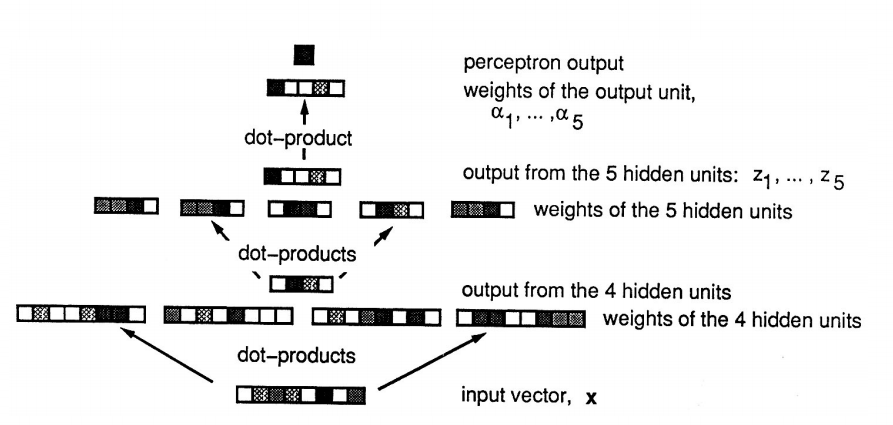
\includegraphics[width=0.6\textwidth]{svm(1).png}
		\caption{具有$8$个输入单元,$2$层隐藏单元和$1$个输出单元的简单前反馈感知机。向量中的灰色阴影反映了它们的数值。}
	\end{figure}

	在Rosenblatt的时代,当时并没有可以通过调整网络的所有权重来最小化向量集误差的算法,而Rosenblatt提出了一种只有输出单元的自适应权重的方法:根据其他权重的设置,将输入向量非线性变换为最后一层单元的特征空间$Z$,在其中构造线性决策函数:
	\begin{equation}
		I(\mathbf{x})=\operatorname{sign}\left(\sum_{i} \alpha_{i} z_{i}(\mathbf{x})\right)\tag{4}
	\end{equation}
	通过对第$i$个隐藏单元到输出单元的权重$a_i$进行调整,以最小化训练数据上的一些误差。作为Rosenblatt方法的结论,决策函数的构造再次与空间中线性超平面的构造产生了联系。

	在1986年发现了一种算法,可以对神经网络的所有权重进行局部调整,以最大程度地减小属于模式识别问题的一组向量上的误差~\upcite{rumelhart1985learning}~\upcite{rumelhart1986learning}~\upcite{parker1985learning}~\upcite{lecun1985procedure},即反向传播算法。该方法涉及了对神经元数学模型的轻微修正,从此神经网络实现了“分段线性型”决策函数。

	在本文中,我们构造了一种新型的学习机,即支持向量网络。支持向量网络实现了以下想法:使用先验选择的一些非线性映射,将输入向量映射到高维特征空间$Z$中,并构造具有特殊性质的线性决策面,以确保网络的强泛化能力。

	例子:为了获得与二阶多项式相对应的决策面,可以构造特征空间$Z$,它有$N=\frac{n(n+3)}{2}$个坐标:
	\begin{align}
		z_{1}&=x_{1},\ldots,z_{n}=x_{n},\quad n \quad coordinates, \notag \\ 
		z_{n+1}&=x_{1}^{2},\ldots,z_{2n}=x_{n}^{2},\quad n\quad coordinates, \notag \\
		z_{2n+1}&=x_{1} x_{2},\ldots,z_{N}=x_{n} x_{n-1},\quad \frac{n(n-1)}{2} \quad coordinates,\notag
	\end{align}
	其中$x=(x_1,\ldots,x_n)$,超平面就在其中被构造。

	上述方法有两个问题:一个是概念上的,另一个是技术上的。概念上的问题是如何找到一个可以很好地泛化的分割超平面:特征空间的维数将是巨大的,且并非所有分割训练数据的超平面都能够很好地泛化$^2$。技术上的问题是如何在计算上处理此类高维空间:如果要在$200$维空间中构造$4$或$5$阶多项式,可能需要在十亿维特征空间中构造超平面。
	\begin{figure}[htbp]
		\centering
		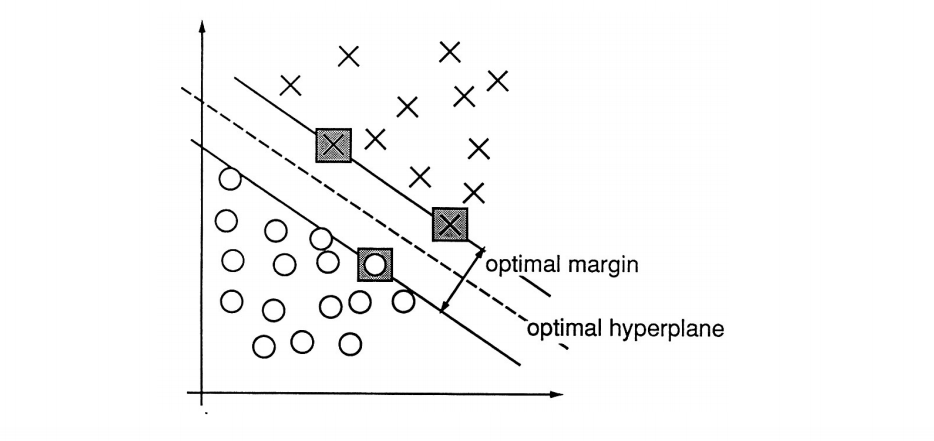
\includegraphics[width=0.6\textwidth]{svm(2).png}
		\caption{二维空间中可分割问题的示例。用灰色正方形标记的支持向量决定了两个类别之间的最大间隔。}
	\end{figure}

	对于此类问题,概念部分于1965年得到解决~\upcite{vapnik1982estimation}。此处将最优超平面定义为线性决策函数,使得在两类向量之间具有最大间隔,见图2。并观察到,构造此类最优超平面时,只需考虑少量训练数据,即确定该间隔的支持向量。其结果表明,如果训练向量被最优超平面无误差地分割,则在测试示例上犯错的概率的期望将受到支持向量数量的期望与训练向量数量之间比例的限制:
	\begin{equation}
		E[\mathrm{Pr}(\mathrm{error})] \leq \frac{E[\text { number of support vectors }]}{\text { number of training vectors }}\tag{5}
	\end{equation}
	注意,此上界不包含间隔空间的维数。可以得出结论:如果可以从相对于训练集大小的少数支持向量构造最优超平面,那么即使在无限维空间中,泛化能力也会很强。在第5节中,我们将证明现实问题的比例(5)可以低至$0.03$,且最优超平面能够在十亿维空间中很好地泛化。

	令
	\begin{equation}
		\mathbf{w}_0·\mathbf{z}+\mathbf{b}_0 =0\notag
	\end{equation}
	为特征空间中的最优超平面。我们将证明特征空间中的最优超平面的权重$\mathbf{w}_0$可以写成一些支持向量的线性组合
	\begin{equation}
		\mathbf{w}_0=\sum_\mathrm{support\ vectors}\alpha_i\mathbf{z}_i\tag{6}
	\end{equation}
	特征空间中的线性决策函数$I(\mathbf{z})$可以写作:
	\begin{equation}
		I(\mathbf{z})=\left(\sum_\mathrm{support\ vectors}\alpha_i\mathbf{z}_i·\mathbf{z}+b_0\right)\tag{7}
	\end{equation}
	其中$\mathbf{z}_i·\mathbf{z}$是支持向量$\mathbf{z}_i$和向量$\mathbf{z}$在特征空间中的点积。因此,决策函数可以描述为两层网络(图3)。
	\begin{figure}[htbp]
		\centering
		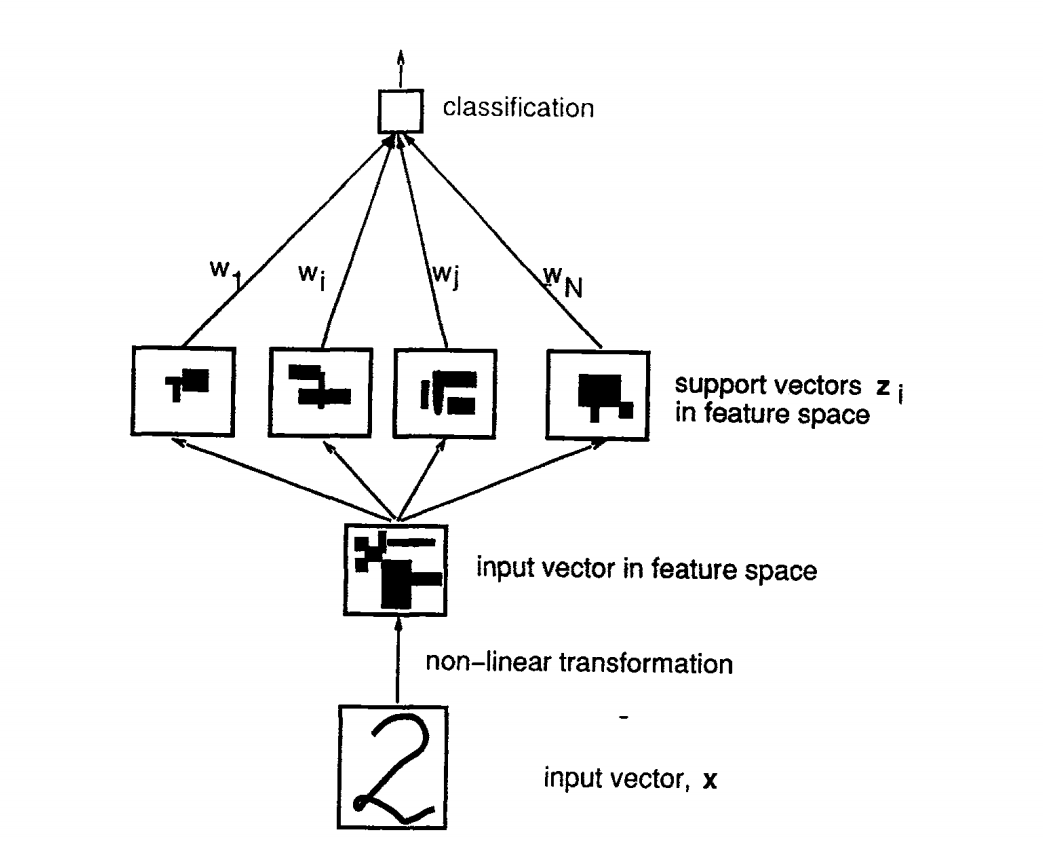
\includegraphics[width=0.6\textwidth]{svm(3).png}
		\caption{从概念上说,通过支持向量网络对未知模式进行分类是通过先将模式变换为一些高维特征空间来完成的,在其中构造的最优超平面决定了输出。与图1相比,可以看到与两层感知机之间的相似性。}
	\end{figure}

	然而,即使最优超平面能够很好地泛化,处理高维特征空间的技术问题仍然存在。
	在1992年证明了:可以交换构造决策函数的操作顺序~\upcite{boser1992training},以代替对输入向量进行非线性变换,然后在特征空间中对带有支持向量的点积进行变换,即能够先比较输入空间中的两个向量(例如将它们的点积或某种距离度量进行比较),然后对结果的值进行非线性变换(见图4)。这使得我们能够构造多种类型的决策面,例如任意阶的多项式决策面。我们将这种学习机称为支持向量网络$^3$。
	\begin{figure}[htbp]
		\centering
		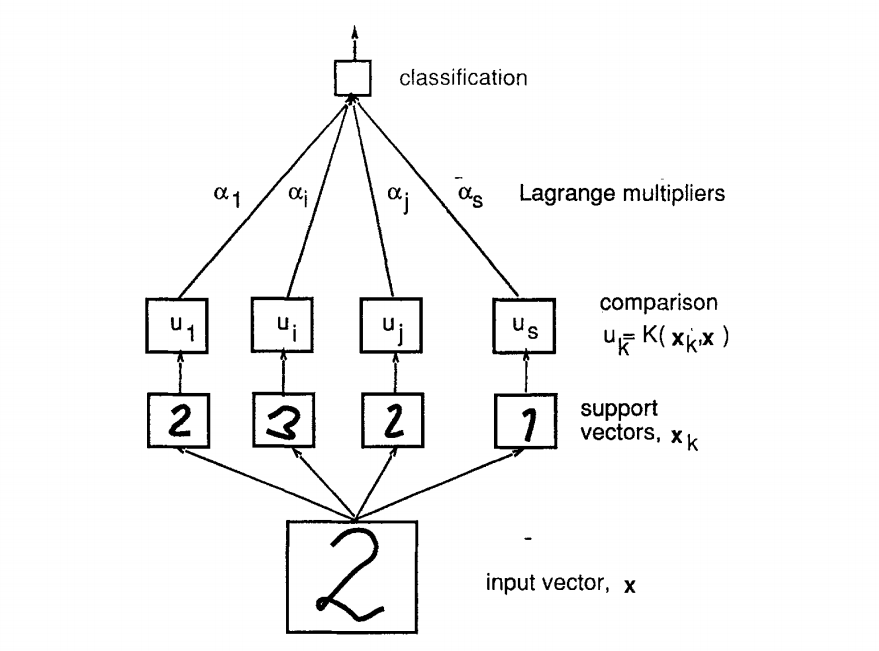
\includegraphics[width=0.6\textwidth]{svm(4).png}
		\caption{支持向量网络对未知模式的分类。与支持向量相比,该模式在输入空间中,结果的值被非线性变换。这些变换值的线性函数确定分类器的输出。}
	\end{figure}

	支持向量网络方法最初是针对在没有误差的情况下分割训练数据的有限情况而开发的。在本文中,我们将推广支持向量网络的用途,以涵盖不可能没有误差地分割训练数据的情况。通过这种推广,我们将支持向量网络视为一种新的学习机,与神经网络一样强大且通用。在第5节中,我们将展示它在高维空间($256$维)中,高阶多项式决策面(至多$7$阶)的泛化效果。并将算法的性能与经典学习机的性能进行比较,例如线性分类器、$k$-近邻分类器和神经网络。第2、3和4节介绍算法的推导要点,并讨论其特性。详细信息参见附录。

	\section{最优超平面}
	在本节中,我们将回顾在无误差地分割训练数据的任务中构造最优超平面的方法~\upcite{vapnik1982estimation}。在下一节中,我们将介绍软间隔的概念,这会允许我们对存在误差的训练集进行分析处理。
	\subsection{最优超平面算法}
	标记过的训练模式集
	\begin{equation}
		(y_1,\mathbf{x}_1),\ldots,(y_\ell,\mathbf{x}_\ell),\qquad y_i\in\{-1,1\}\tag{8}
	\end{equation}
	被称为线性可分的,即如果存在一个向量$\mathbf{w}$和一个标量$b$使得以下不等式
	\begin{align}
		\mathbf{w}·\mathbf{x}_i+b\geq1\qquad if\quad y_i=1,\notag \\
		\mathbf{w}·\mathbf{x}_i+b\leq-1\qquad if\quad y_i=-1,\tag{9}
	\end{align}
	对训练集(8)的所有元素成立。下面我们将(9)写成另一种形式$^4$:
	\begin{equation}
		y_i(\mathbf{w}·\mathbf{x}_i+b)\geq1,\qquad i=1,\ldots,\ell.\tag{10}
	\end{equation}

	最优超平面
	\begin{equation}
		\mathbf{w_0·x}+b_0=0\tag{11}
	\end{equation}
	是唯一一个以最大间隔分割训练数据的:回想一下图2,它确定了方向$\mathbf{w}/|\mathbf{w}|$,使得两个不同类别训练向量投影之间的距离最大。距离$\rho(\mathbf{w},b)$由以下公式给出:
	\begin{equation}
		\rho(\mathbf{w},b)=\min_{\{\mathbf{x}:y=1\}}\frac{\mathbf{x·w}}{|\mathbf{w}|}-\max_{\{\mathbf{x}:y=-1\}}\frac{\mathbf{x·w}}{|\mathbf{w}|}\tag{12}.
	\end{equation}
	最优超平面$(\mathbf{w}_0,b_0)$是使距离(12)最大化的参数。由(10)和(12)得到
	\begin{equation}
		\rho(\mathbf{w}_0,b_0)=\frac{2}{|\mathbf{w}_0|}=\frac{2}{\sqrt{\mathbf{w}_0·\mathbf{w}_0}}.\tag{13}
	\end{equation}
	这意味着最优超平面是在约束(10)下最小化$\mathbf{w·w}$的唯一平面。因此,构造最优超平面成为了一个二次规划问题。

	$y_i(\mathbf{w}·\mathbf{x}_i+b)=1$中的向量$\mathbf{x}_i$称为支持向量。在附录A.1中我们证明了确定最优超平面的向量$\mathbf{w}_0$可以表示为训练向量的线性组合:
	\begin{equation}
		\mathbf{w}_0=\sum_{i=1}^{\ell}{y_i\alpha_i^0\mathbf{x}_i}\tag{14}
	\end{equation}
	其中$\alpha_i^0\geq0$。由于$\alpha>0$仅适用于支持向量(见附录),所以表达式(14)呈现了$\mathbf{w}_0$的紧凑形式。
	我们还表明了为了找到参数$\alpha_i$的向量:
	\begin{equation}
		\mathbf{\Lambda}_0^T=(\alpha_1^0,\dots,\alpha_\ell^0),\notag
	\end{equation}
	必须解决以下的二次规划问题:
	\begin{equation}
		W(\mathbf{\Lambda})=\mathbf{\Lambda}^T\mathbf{1}-\frac{1}{2}\mathbf{\Lambda}^T\mathbf{D\Lambda}\tag{15}
	\end{equation}
	其中$\mathbf{\Lambda}^T=(\alpha_1,\dots,\alpha_\ell)$,并受约束:
	\begin{align}
		\mathbf{\Lambda}\geq\mathbf{0},\tag{16}\\ 
		\mathbf{\Lambda}^T\mathbf{Y}=0,\tag{17}
	\end{align}
	其中$\mathbf{1}^T=(1,\dots,1)$是$\ell$-维单位向量,$\mathbf{Y}^T=(y_1,\dots,y_\ell)$是$\ell$-维标签向量,$\mathbf{D}$是对称的$\ell\times\ell$矩阵,元素为
	\begin{equation}
		D_{ij}=y_iy_j\mathbf{x}_i·\mathbf{x}_j,\quad i,j=1,\dots,l.\tag{18}
	\end{equation}
	不等式(16)表明了非负性。因此,在(17)的约束下,我们必须在非负区域中最大化二次型(15)。

	当训练数据(8)可以无误差地分割时,我们在附录A中展示了函数(15)的最大值,$(\mathbf{\Lambda}_0,b_0)$和(13)中的最大间隔$\rho_0$有如下关系:
	\begin{equation}
		W(\mathbf{\Lambda}_0)=\frac{2}{\rho_0^2}.\tag{19}
	\end{equation}
	如果对于一些$\mathbf{\Lambda}_*$和大常数$W_0$不等式
	\begin{equation}
		W(\mathbf{\Lambda}_*)> W_0\tag{20}
	\end{equation}
	成立,那么可以断言,所有将训练数据(8)分割的超平面都具有间隔
	\begin{equation}
		\rho< \sqrt{\frac{2}{W_0}}.\notag
	\end{equation}
	如果训练集(8)无法通过超平面分割,那么两类模式之间的间隔会变得任意小,从而导致函数$W(\mathbf{\Lambda})$的值变得任意大。因此,在约束(16)和(17)下使函数(15)最大化,一个要么达到最大值(在这种情况下,可以用最大间隔$\rho_0$构造超平面),要么发现最大值超过了某个给定的(大)常数$W_0$(在这种情况下,不可能以大于$\sqrt{2/W_0}$的间隔分割训练数据)。

	利用以下方法可以非常有效地解决在约束(16)和(17)下最大化函数(15)的问题。即将训练数据划分为多个部分,每个部分中的训练向量数应尽可能少。首先解决由训练数据的第一部分确定的二次规划问题,对于此问题,有两种可能的结果:一是无法通过超平面分割数据的这一部分(在这种情况下,也无法分割整个数据集),而是找到了用于分割训练数据的第一部分的最优超平面。

	令在能够分割第一部分的情况下使函数(15)最大化的向量为$\mathbf{\Lambda}_1$,$\mathbf{\Lambda}_1$的部分坐标为$0$,对应于该部分的非支持训练向量。生成一组新的训练数据,其中包含来自训练数据第一部分的支持向量和不满足约束(10)的第二部分向量,其中$\mathbf{w}$由$\mathbf{\Lambda}_1$确定。对于此集合,构造一个新函数$W_2(\mathbf{\Lambda})$并令其在$\mathbf{\Lambda}_2$处最大化。继续逐步构造覆盖训练数据所有部分的解向量$\mathbf{\Lambda}_*$,要么发现不可能无误差地分割训练集,要么构造出针对整个数据集的最优分割超平面$\mathbf{\Lambda}_*=\mathbf{\Lambda}_0$。注意,在此过程中,函数$W(\mathbf{\Lambda})$的值单调增加,因为在优化过程中考虑了越来越多的训练向量,导致两类之间的间隔越来越小。

	\section{软间隔超平面}
	再考虑不可能无误差地分割训练数据的情况。在这种情况下,我们希望以最少的误差数来分割训练集。为了证明这一点,让我们展示一些非负变量$\xi\geq0,i=1,\dots,\ell$。

	现在我们可以最小化函数
	\begin{equation}
		\Phi(\xi)=\sum_{i=1}^\ell\xi_i^\sigma\tag{21}
	\end{equation}
	对于较小的$\sigma>0$,受约束
	\begin{align}
		y_i(\mathbf{w}·\mathbf{x}_i+b) \geq 1-\xi_i,\quad i=1,\dots,\ell, \tag{22} \\
		\xi_i \geq 0,\quad \qquad i=1,\dots,\ell.\tag{23}
	\end{align}
	如果$\sigma$足够小,函数(21)则描述了训练误差的数量$^5$。

	最小化(21)可以找到一些训练误差的最小子集:
	\begin{equation}
		(y_{i_1},\mathbf{x}_{i_1}),\dots,(y_{i_k},\mathbf{x}_{i_k}).\notag
	\end{equation}
	如果将这些数据从训练集中移除,则可以无误差地将训练集中的其余部分分割,则可以构造最优分割超平面。

	这个想法可以表示为:最小化函数
	\begin{equation}
		\frac{1}{2}\mathbf{w}^2+CF\left(\sum_{i=1}^{\ell}\xi_i^\sigma\right)\tag{24}
	\end{equation}
	受约束(22)和(23),其中$F(u)$是单调凸函数,$C$是常数。

	对于足够大的$C$和足够小的$\sigma$,在约束(22)和(23)下将函数(24)最小化的向量$\mathbf{w}_0$和常数$b_0$,确定了能够将训练集上的误差数最小化的超平面,并用最大间隔分割了其余部分元素。

	但是请注意,构造一个使训练集上的误差数量最小化的问题通常是$NP$-完全的。为了避免问题的$NP$-完全性,我们将考虑$\sigma=1$的情况(优化问题(15)具有唯一解的$\sigma$的最小值)。其中,函数(24)描述了(对于足够大的$C$而言)构造分割超平面的问题,该分割超平面最小化了训练误差的偏差之和,并最大化了正确分类的向量的间隔。如果可以无误差地分割训练数据,则构造的超平面将与最优分割超平面重合。

	与$\sigma<1$的情况相反,存在一种在$\sigma=1$的情况下找到(24)的解的有效方法,我们称之为软间隔超平面。

	在附录A中我们考虑了最小化函数
	\begin{equation}
		\frac{1}{2}\mathbf{w}^2+CF\left(\sum_{i=1}^{\ell}\xi_i\right)\tag{25}
	\end{equation}
	受约束(22)和(23),其中$F(u)$是单调凸函数且$F(0)=0$。为了简化公式,我们在本节中仅描述$F(u)=u^2$的情况。对于此函数,优化问题仍然是二次规划问题。

	在附录A中,我们证明了,对于最优超平面算法,向量$\mathbf{w}$可以写成支持向量$\mathbf{x}$的线性组合:
	\begin{equation}
		\mathbf{w}_0=\sum_{i=1}^{\ell}\alpha_i^0y_i\mathbf{x}_i.\notag
	\end{equation}
	为了找到向量$\mathbf{\Lambda}^T=(\alpha_1,\dots,\alpha_{\ell})$,必须解决最大化对偶二次规划问题
	\begin{equation}
		W(\mathbf{\Lambda,\delta})=\mathbf{\Lambda}^T\mathbf{1}-\frac{1}{2}\left[\mathbf{\Lambda}^T\mathbf{D\Lambda}+\frac{\delta^2}{C}\right]\tag{26}
	\end{equation}
	受约束
	\begin{align}
		\mathbf{\Lambda}^T\mathbf{Y}=0,\tag{27} \\
		\delta\geq0,\tag{28} \\
		\mathbf{0}\leq\mathbf{\Lambda}\leq\delta\mathbf{1},\tag{29}
	\end{align}
	其中$\mathbf{1}$,$\mathbf{\Lambda}$,$\mathbf{Y}$,和$\mathbf{D}$与用于构造最优超平面的优化问题中使用的元素相同,而且$\delta$是标量,并且(29)是一个向量不等式。

	注意,(29)表明函数(26)中允许的最小$\delta$值为
	\begin{equation}
		\delta=\alpha_\mathrm{max}=\max(\alpha_1,\dots,\alpha_{\ell}).\notag
	\end{equation}
	因此,为了找到一个软间隔分类器,必须找到一个向量$\mathbf{\Lambda}$最大化
	\begin{equation}
		W(\mathbf{\Lambda})=\mathbf{\Lambda}^T\mathbf{1}-\frac{1}{2}\left[\mathbf{\Lambda}^T\mathbf{D\Lambda}+\frac{\alpha_{\mathrm{max}}^2}{C}\right]\tag{30}
	\end{equation}
	受约束$\mathbf{\Lambda}>\mathbf{0}$和(27)。该问题与仅通过函数(30)中具有最大值的余项来构造最优间隔分类器的问题不同。因此,构造软间隔分类器的问题的解决方法是唯一的,并且对任意数据集都通用。

	由于带有$\alpha_\mathrm{max}$的余项,所以函数(30)不是二次的。在约束$\mathbf{\Lambda}>\mathbf{0}$和(27)的情况下最大化(30),属于所谓的凸规划问题。因此,构造一个软间隔分类器既可以解决参数$\mathbf{\Lambda}$在$\ell$-维空间中的凸规划问题,也可以解决$\mathbf{\Lambda}$在$S$的对偶$\ell+1$空间的二次规划问题。我们的实验通过解决对偶二次规划问题构造了软间隔超平面。

	\section{点积在特征空间中的卷积方法}
	前面各节中描述的算法都在输入空间中构造了超平面,首先必须通过选择$N$-维向量函数$\phi$将$n$-维输入向量$\mathbf{x}$变换为$N$-维特征向量:
	\begin{equation}
		\phi:\mathfrak{R}^n\to\mathfrak{R}^N.\notag
	\end{equation}
	然后为这组变换向量构造一个$N$-维线性分割$\mathbf{w}$和一个偏置$b$
	\begin{equation}
		\phi(\mathbf{x}_i)=\phi_1(\mathbf{x}_i),\phi_2(\mathbf{x}_i),\dots,\phi_N(\mathbf{x}_i),\qquad i=1,\dots,\ell\notag
	\end{equation}
	未知向量$\mathbf{x}$的分类是通过首先将向量变换到分割空间$(\mathbf{x}\mapsto\phi(\mathbf{x}))$,然后取函数的符号来完成的
	\begin{equation}
		f(\mathbf{x})=\mathbf{w}·\phi(\mathbf{x})+b.\tag{31}
	\end{equation}

	根据软间隔分类器方法的性质,向量$\mathbf{w}$可以表示为支持向量的线性组合(在特征空间中)。这意味着
	\begin{equation}
		\mathbf{w}=\sum_{i=1}^{\ell}y_i\alpha_i\phi(\mathbf{x}_i)\tag{32}
	\end{equation}
	点积的线性性质表明,(31)中未知向量$\mathbf{x}$的分类函数$f$只与点积有关:
	\begin{equation}
		f(\mathbf{x})=\phi(\mathbf{x})·\mathbf{w}+b=\sum_{i=1}^{\ell}y_i\alpha_i\phi(\mathbf{x})·\phi(\mathbf{x}_i)+b.\tag{33}
	\end{equation}
	构造支持向量网络的想法来自于,考虑Hilbert空间中点积的一般形式~\upcite{anderson1962classification}:
	\begin{equation}
		\phi(\mathbf{u})·\phi(\mathbf{v})\equiv K(\mathbf{u},\mathbf{v})\tag{34}
	\end{equation}
	根据Hilbert-Schmidt理论~\upcite{courant1953methods},任何对称函数$K(\mathbf{u},\mathbf{v})\in L_2$,都可以展开为
	\begin{equation}
		K(\mathbf{u},\mathbf{v})=\sum_{i=1}^\infty\lambda_i\phi_i(\mathbf{u})·\phi_i(\mathbf{v}),\tag{35}
	\end{equation}
	其中$\lambda_i\in\mathfrak{R}$和$\phi_i$是特征值和特征函数
	\begin{equation}
		\int K(\mathbf{u},\mathbf{v}) \phi_i(\mathbf{u})d\mathbf{u} = \lambda_i \phi_i(\mathbf{v}). \notag
	\end{equation}
	在积分下被内核$K(\mathbf{u},\mathbf{v})$所定义。能确保(34)定义了特征空间中一种点积的充分条件是,在展开式(35)中所有特征值都是正的。为了确保这些系数都是正的,以下是充分必要条件(Mercer‘s 理论),即
	\begin{equation}
		\int \int K(\mathbf{u},\mathbf{v})g(\mathbf{u})g(\mathbf{v})d\mathbf{u}d\mathbf{v}>0 \notag
	\end{equation}
	对所有这样的$g$均满足
	\begin{equation}
		\int g^2(\mathbf{u})d\mathbf{u}<\infty.\notag
	\end{equation}
	因此,满足Mercer‘s理论的函数可以被用作点积。Aizerman,Braverman和Rozonoer(1964)考虑了特征空间中点积的一种卷积~\upcite{aizerman1964theoretical},卷积函数为
	\begin{equation}
		K(\mathbf{u},\mathbf{v})=\mathrm{exp}\left(-\frac{|\mathbf{u}-\mathbf{v}|}{\sigma}\right),\tag{36}
	\end{equation}
	被他们称为势函数。

	然而,特征空间中点积的卷积可以被任意满足Mercer’s调节的函数给出;特别地,为了在$n$维输入空间中构造$d$阶多项式分类器,可以使用以下函数
	\begin{equation}
		K(\mathbf{u},\mathbf{v})=(\mathbf{u}·\mathbf{v}+1)^d.\tag{37}
	\end{equation}
	使用不同的点积$K(\mathbf{u},\mathbf{v})$能够构造有任意类型决策面的学习机~\upcite{boser1992training}。决策面有这样的形式
	\begin{equation}
		f(\mathbf{x})=\sum_{i=1}^{\ell}y_i\alpha_iK(\mathbf{x},\mathbf{x}_i),\notag
	\end{equation}
	其中$\mathbf{x}_i$是支持向量在输入空间中的像,且$\alpha_i$是支持向量在特征空间中的权重。

	为了找到向量$\mathbf{x}_i$和权重$\alpha_i$,可以遵循相同的关于原最优间隔分类器或软间隔分类器的解决方法。唯一的差别是矩阵$D$(被(18)确定),另一个则使用矩阵
	\begin{equation}
		D_{ij}=y_iy_jK(\mathbf{x}_i,\mathbf{x}_j),\quad i,j=1,\dots,l.\notag
	\end{equation}

	\section{支持向量网络的一般特性}
	\subsection{通过支持向量网络构造决策规则是高效的}
	为了构造支持向量网络决策规则,必须解决以下二次最优化问题:
	\begin{equation}
		W(\mathbf{\Lambda,\delta})=\mathbf{\Lambda}^T\mathbf{1}-\frac{1}{2}\left[\mathbf{\Lambda}^T\mathbf{D\Lambda}+\frac{\delta^2}{C}\right],\notag
	\end{equation}
	受约束:
	\begin{align}
		\mathbf{0}\leq\mathbf{\Lambda}\leq\delta\mathbf{1}, \notag \\
		\mathbf{\Lambda}^T\mathbf{Y}=0,\notag
	\end{align}
	其中矩阵
	\begin{equation}
		D_{ij}=y_iy_jK(\mathbf{x}_i,\mathbf{x}_j),\quad i,j=1,\dots,l.\notag
	\end{equation}
	被训练集的元素所定义,且$K(\mathbf{u},\mathbf{v})$是决定点积的卷积函数。

	通过解决由训练数据确定的当前构成支持向量的间接优化问题,可以有效地找到优化问题的解决方法。第3节中介绍了此方法,获得的最优决策函数也是唯一的$^6$。

	这意味着我们可以使用任意标准技巧来解决任意优化问题。

	\subsection{支持向量网络是一种通用机}
	通过更改决定点积的卷积函数$K(\mathbf{u},\mathbf{v})$可以获得不同的网络。

	在下一节中我们将考虑使用多项式决策面的支持向量网络。为了指明不同阶的多项式,可以使用下列点积的卷积函数
	\begin{equation}
		K(\mathbf{u},\mathbf{v})=(\mathbf{u}·\mathbf{v}+1)^d.\notag
	\end{equation}
	径向基函数机有决策函数
	\begin{equation}
		f(\mathbf{x})=\mathrm{sign}\left(\sum_{i=1}^n \mathrm{exp}\left\{\frac{|\mathbf{x}-\mathbf{x}_i|^2}{\sigma^2}\right\}\right) \notag
	\end{equation}
	可以使用以下的卷积函数实现
	\begin{equation}
		K(\mathbf{u},\mathbf{v})=\mathrm{exp}\left\{-\frac{|\mathbf{u}-\mathbf{v}|^2}{\sigma^2}\right\}. \notag
	\end{equation}
	在这种情况下,支持向量网络机将构造出近似函数的中心$\mathbf{x}_i$和权重$\alpha_i$。

	通过构造特殊的卷积函数,还可以结合当前问题的先验知识。因此,支持向量网络是一种相当通用的学习机,可以很简单地通过改变点积形式来改变决策函数集。

	\subsection{支持向量网络与泛化能力控制}
	要控制学习机的泛化能力,必须控制两个不同的因子:训练数据的误差率和通过$VC$-维所测量的学习机的能力~\upcite{vapnik1982estimation}。在测试集上存在的误差率有以下形式的界限:有$1-\eta$的概率,不等式
	\begin{equation}
		\mathrm{Pr(test\ error)\leq Frequency(training\ error)+Confidence\ Interval} \tag{38}
	\end{equation}
	成立。在界限(38)中,置信区间取决于学习机的$VC$-维,训练集中的元素数量以及$\eta$的值。

	(38)中的两个因子形成了一种相互制约:学习机函数集的$VC$-维越小,置信区间越小,但错误频率的值越大。

	解决这种相互制约的一般方法被提出为结构风险最小化原理:对于给定的数据集,必须找到一种使其总和最小化的解决方法。它的特殊情况是奥卡姆剃刀原理:保持第一项为零,并最小化第二项。

	已知线性指标函数集的$VC$-维
	\begin{equation}
		I(\mathbf{x})=\mathrm{sign}(\mathbf{w}·\mathbf{x}+b),\quad |\mathbf{x}|\leq C_\mathbf{x} \notag
	\end{equation}
	其中固定阈值$b$等于输入空间维数。然而,子集的$VC$-维
	\begin{equation}
		I(\mathbf{x})=\mathrm{sign}(\mathbf{w}·\mathbf{x}+b),\quad |\mathbf{x}|\leq C,\quad |\mathbf{w}|\leq C_\mathbf{w} \notag
	\end{equation}
	(具有权重的有界函数的函数集)可以小于输入空间的维数,取决于$C_\mathbf{w}$。

	从这个角度看,最优间隔分类器遵循奥卡姆剃刀原理。他使(38)的第一项为零(通过满足不等式(9)),并且使第二项最小化(通过使函数$\mathbf{w}·\mathbf{w}$最小化),这种最小化可以防止过拟合的问题。

	然而,即使在训练数据可分割的情况下,也可以通过使(38)中的置信度最小化来获得更好的泛化能力,甚至代价是训练集的误差。在软间隔分类器方法中,则可以通过选择适当的参数$C$来完成。在支持向量网络算法中,在更普遍的情况,即训练集上不存在零误差的解决方法,则是通过更改参数$C$来权衡决策规则的复杂性和误差率。因此,支持向量网络可以控制学习机泛化能力的两个因子。

	\section{实验分析}
	为了演示支持向量网络方法,我们进行了两种类型的实验。我们在平面上生成任意构造的模式集,并使用二阶多项式决策面进行实验,再对数字识别的实际问题进行实验。

	\subsection{平面实验}
	利用以下形式的点积
	\begin{equation}
		K(\mathbf{u},\mathbf{v})=(\mathbf{u}·\mathbf{v}+1)^d \tag{39}
	\end{equation}
	$d=2$,我们为平面中的不同模式集构造决策规则。这些实验的结果可以可视化,并且可以很好地说明算法的功能,见图5。这两个类别分别由黑白符号表示。在图中,我们用圆圈表示支持模式,而用交叉表示误差。在不存在使得误差更少的二阶多项式的情况下,该解决方法是最优的。注意,相对于训练模式的数量,支持模式的数量很小。
	\begin{figure}[htbp]
		\centering
		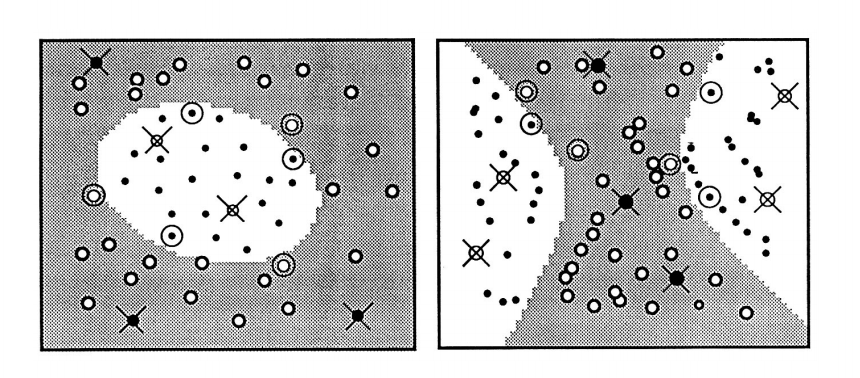
\includegraphics[width=0.6\textwidth]{svm(5).png}
		\caption{$d=2$时点积(39)的示例。圆圈表示支持模式,交叉表示误差。}
	\end{figure}

	\subsection{数字识别实验}
	构造支持向量网络的实验利用了两个不同的数据库进行位图数字识别,即一个小型数据库和大型数据库。较小的是美国邮政服务数据库,其中包含$7300$种训练模式和$2000$种测试模型。该数据库的分辨率为$16\times16$像素,一些示例如图6所示。在该数据库上,我们进行了各阶多项式的实验研究。
	\begin{figure}[htbp]
		\centering
		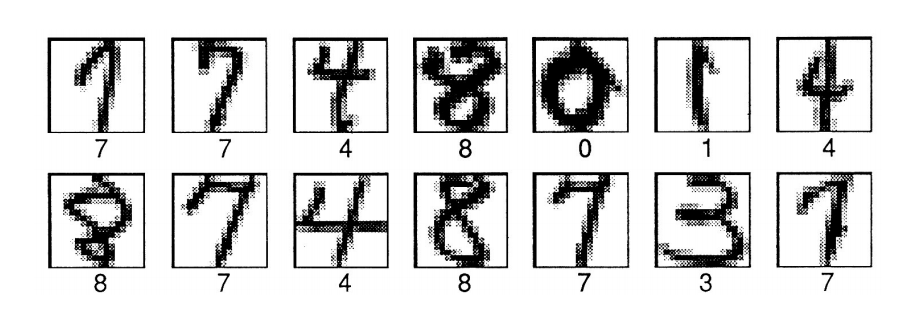
\includegraphics[width=0.6\textwidth]{svm(6).png}
		\caption{美国邮政服务数字数据库中带有标签的模式示例。}
	\end{figure}
	大型数据库包含$60000$个训练模式和$10000$个测试模式,并且是NIST$^7$训练集和测试集的50-50混合。这些模式的分辨率为$28\times28$,产生的输入维度为$784$。在此数据库上,我们仅构造了$4$次多项式分类器。然后将该分类器的性能与参加基准研究的其他类型的学习机进行比较~\upcite{bottou1994comparison}。

	在我们所有的实验中,构造了十个分割,每个类别一个。每个超平面都使用相同的点积和数据预处理。根据这十个分类器的最大输出完成未知模式的分类。

	\subsubsection{美国邮政服务数据库实验}
	美国邮政服务数据库使用了真实邮件,这已被其他研究人员报告过。在表1中,我们列出了从文献和实验中收集的各种分类器的性能数据。J. Bromley&E. Sackinger报告了人类的表现结果~\upcite{bromley1991neural}。$CART$的结果由新泽西州Murray Hill,贝尔实验室的Daryl Pregibon和Michale D. Riley给出。本文中,由Corinna Cortes和Bernard Schoelkopf分别获得了$C4.5$和最优$2$层神经网络(最优隐藏单元数)的结果。而Y. LeCun等人获得了具有$5$层专用神经网络架构LeNet1的结果~\upcite{lecun1990handwritten}。
	\begin{table}[!htbp]
		\centering
		\caption{来自出版物和自己实验的各种分类器的性能数据。参考资料。}
		\begin{tabular}{lc}
			\hline 
			{\text { Classifier }} & {Raw\ error,\%} \\ 
			\hline 
			{\text { Human performance }} & {2.5} \\ 
			{\text { Decision tree, CART }} & {17} \\ 
			{\text { Decision tree, C4.5 }} & {17} \\ 
			{\text { Best 2 layer neural network }} & {6.6} \\ 
			{\text { Special architecture 5 layer network }} & {5.1} \\ 
			\hline
		\end{tabular}
	\end{table}
	在使用美国邮政服务数据库进行的实验中,我们进行了数据预处理(居中,倾斜和平滑),以结合目前有关问题不变性的知识。~\cite{boser1992training}中Boser研究了数据平滑对支持向量网络的影响。对于实验,我们选择高斯平滑内核,标准差$\sigma=0.75$,与~\cite{boser1992training}一致。

	基于形式(39)的点积,输入维数为$256$,多项式的阶数范围为$1$到$7$。表2呈现了实验结果,训练数据不是线性可分的。
	\begin{table}[!htbp]
		\centering
		\caption{不同阶数的多项式的点积获得的结果。“支持向量”的数量是每个分类器的平均值。}
		\begin{tabular}{cccc}
			\hline 
			\text { Degree of } & {\text { Raw }} & {\text { Support }} & {\text { Dimensionality of }} \\
			\text { polynomial } & {\text { error, } \%} & {\text { vectors }} & {\text { feature space }} \\
			\hline 
			{1} & {12.0} & {200} & {256} \\
			{2} & {4.7} & {127} & {$\sim 33000$} \\
			{3} & {4.3} & {148} & {$\sim 1 \times 10^{6}$} \\
			{4} & {4.3} & {175} & {$\sim 1 \times 10^{9}$} \\
			{5} & {4.3} & {175} & {$\sim 1 \times 10^{12}$} \\
			{6} & {4.2} & {185} & {$\sim 1 \times 10^{14}$} \\
			{7} & {4.3} & {190} & {$\sim 1 \times 10^{16}$} \\
			\hline
		\end{tabular}
	\end{table}
	请注意,支持向量的数目增加得非常缓慢。$7$阶多项式得支持向量仅比$3$阶多项式多$30\%$,甚至少于$1$阶多项式。然而,用于$7$阶多项式分类器的特征空间维数比用于$3$阶多项式分类器的大$1010$倍。再次注意,性能几乎不会随着空间维数的增加而改变,这说明没有过拟合的问题。

	线性分割的支持向量数量相对较高是由于其不可分割性:数字$200$包含了支持向量和具有非零$\xi$-值的训练向量。如果$\xi>1$的训练向量被错误分类,在线性情况下,训练集上的错误分类次数则为平均$34$次每分类器。对于$2$阶分类器,训练集上的错误分类次数降低到$4$。这$4$种分类错误的模式如图7所示。
	\begin{figure}[htbp]
		\centering
		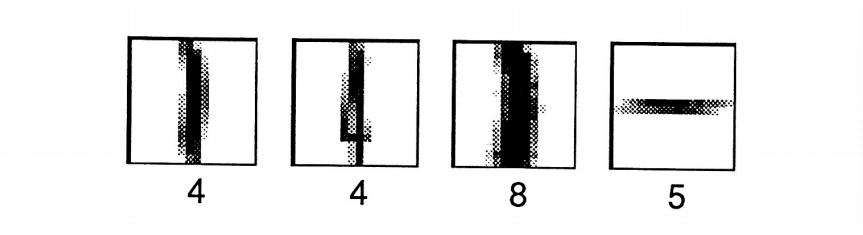
\includegraphics[width=0.6\textwidth]{svm(7).png}
		\caption{标注的$2$阶多项式支持向量分类器在训练集上出错的示例。}
	\end{figure}
	值得注意的是,在我们所有的实验中,当我们考虑获得的支持向量数量而不是该数量的期望值时,泛化能力的上限(5)成立。即单个分类器的错误概率上限不超过$3\%$(在测试数据上,单个分类器的实际误差不超过$1.5\%$)。

	构造多项式分类器的训练时间不取决于多项式的阶数,而仅取决于支持向量的数量。即使在最坏的情况下,它也比性能最好的神经网络LeNet1更快~\upcite{lecun1990handwritten},该神经网络的误差为$5.1\%$,阶数$2$或更高的多项式分类器优于LeNet1。

	\subsubsection{NIST数据库实验}
	NIST数据库仅用于进行了$2$周的基准研究。在有限的时间内,只能构造出一种类型的分类器,因此我们选择了没有进行数据预处理的$4$阶多项式,这基于我们在美国邮政数据库实验中的经验。

	表3列出了$10$个分类器中每个分类器的支持向量的数量,并给出了分类器在训练集和测试集上的性能表现。注意,即使是$4$阶多项式(具有超过$108$个自由参数)在此训练集上也会出错。每个类别的平均训练误差率为$0.02\%\sim12$。图8显示了分类器$1$的$14$个分类错误的测试模式。再次注意,对于获得的支持向量数量,上限(5)是如何成立的。

	\begin{table}[!htbp]
		\centering
		\caption{在NIST数据库上针对$4$阶多项式分类器获得的结果。训练集的大小为$60000$模式,测试集的大小为$10000$模式。}
		\begin{tabular}{ccccccccccc}
			\hline
			{} & {C1.0} & {C1.1} & {C1.2} & {C1.3} & {C1.4} & {C1.5} & {C1.6} & {C1.7} & {C1.8} &{C1.9} \\
			\hline
			{Supp.patt.} & 1379 & 989 & 1958 & 1900 & 1224 & 2024 & 1527 & 2064 & 2332 & 2765 \\
			{Error\ train} & 7 & 16 & 8 & 11 & 2 & 4 & 8 & 16 & 4 & 1 \\
			{Error\ test} & 19 & 14 & 35 & 35 & 36 & 49 & 32 & 43 & 48 & 63 \\
    		\hline
		\end{tabular}
	\end{table}
	\begin{figure}[htbp]
		\centering
		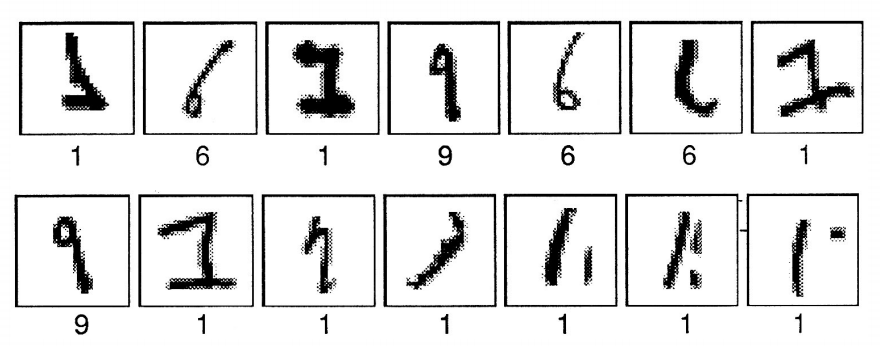
\includegraphics[width=0.6\textwidth]{svm(8).png}
		\caption{分类器$1$分类错误的$14$个带有标签的测试模式。带有标签”$1$“的模式为假阴性,其他的为假阳性。}
	\end{figure}
	测试集上$10$个分类器的综合性能为$1.1\%$误差率。该结果与基准研究种其他参与分类器的结果进行了比较,包括一个线性分类器,一个具有$60000$模式的$k=3$最近邻分类器,以及两个专门为数字识别而构建的神经网络(LeNet1和LeNet4)。作者仅为支持向量网络的结果做出了贡献。基准测试结果如图9所示。
	\begin{figure}[htbp]
		\centering
		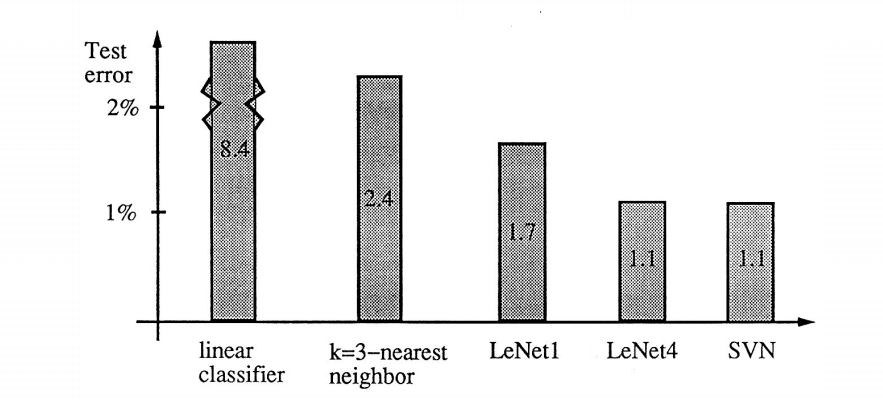
\includegraphics[width=0.6\textwidth]{svm(9).png}
		\caption{来自基准研究的结果。}
	\end{figure}
	我们通过引用描述基准测试结果的论文来结束本节~\upcite{bottou1994comparison}:
	\begin{quote}
		长期以来,LeNet1被一致认为是最新方法…,后通过一系列体系结构实验,结合对识别错误特征的分析,精心设计了LeNet4…

		支持向量网络具有出色的准确性,最值得注意的是,与其他分类器不同,它不包含有关问题几何结构的先验认知。实际上,如果图像像素被加密(例如通过固定的随机的排列),分类器也将做到同样的事情。
	\end{quote}
	最后一句话表明,可以通过构建点积$K(\mathbf{u},\mathbf{v})$的函数来提高支持向量网络的性能,这些函数反映了有关当前问题的先验信息。

	\section{总结}
	这篇论文介绍了作为二分类问题的新学习机—支持向量网络。

	支持向量网络结合了$3$个想法:来自最优超平面的求解方法(允许在支持向量上扩展解向量),点积的卷积想法(将求解表面从线性扩展到非线性)和软间隔的概念(以考虑训练集上的误差)。

	该算法已经经过测试,并与其他经典算法的性能进行了比较。尽管决策面的设计十分简单,但新算法在对比研究中仍表现出非常好的性能。

	其他功能(如容量控制和易于更改已构造的决策面)使支持向量网络成为功能强大且通用的学习机。

	\section*{A. 构造分割超平面}
	在本附录中,我们推导构造最优超平面和软间隔超平面的方法。

	\subsection*{A.1 最优超平面算法}
	在第2节中表明,构造最优超平面
	\begin{equation}
		\mathbf{w_0·x}+b=0\tag{40}
	\end{equation}
	分割训练数据集
	\begin{equation}
		(y_1,\mathbf{x}_1),\ldots,(y_\ell,\mathbf{x}_\ell),\notag
	\end{equation}
	必须最小化函数
	\begin{equation}
		\Phi=\mathbf{w}·\mathbf{w},\notag
	\end{equation}
	受约束
	\begin{equation}
		y_i(\mathbf{x}_i·\mathbf{w}+b)\geq1,\qquad i=1,\ldots,\ell.\tag{41}
	\end{equation}
	为此,我们使用标准的优化方法。我们构造一个拉格朗日函数
	\begin{equation}
		L(\mathbf{w},b,\mathbf{\Lambda})=\frac{1}{2}\mathbf{w}\cdot\mathbf{w}-\sum_{i=1}^\ell\alpha_i[y_i(\mathbf{x}_i\cdot\mathbf{w}+b)-1],\tag{42}
	\end{equation}
	其中$\mathbf{\Lambda}=(\alpha_1,\dots,\alpha_\ell)$对应约束(41)的非负拉格朗日乘子。

	众所周知,最优化问题的结果由$\mathbf{w}$,$\mathbf{\Lambda}$和$b$的$2\ell+1$-维空间中的拉格朗日方程的鞍点确定,其中应相对于参数$\mathbf{w}$和$b$取最小值,并应相对对拉格朗日乘子$\mathbf{\Lambda}$取最大值。

	在最小值(关于$\mathbf{w}$和$b$)的点上,获得:
	\begin{align}
		\left.\frac{\partial L(\mathbf{w},b,\mathbf{\Lambda})}{\partial \mathbf{w}}\right|_{\mathbf{w}=\mathbf{w}_0}&=\left(\mathbf{w}_0-\sum_{i=1}^\ell\alpha_iy_i\mathbf{x}_i \right)=0,\tag{43} \\
		\left.\frac{\partial L(\mathbf{w},b,\mathbf{\Lambda})}{\partial b}\right|_{b=b_0}&=\sum_{\alpha_i}y_i\alpha_i=0.\tag{44}
	\end{align}
	从等式(43)我们得到
	\begin{equation}
		\mathbf{w}_0=\sum_{i=1}^\ell \alpha_i y_i \mathbf{x}_i , \tag{45}
	\end{equation}
	这表明最优超平面可以写成训练向量的线性组合。请注意,只有$\alpha_i>0$的训练向量$\mathbf{x}$对总和(45)有贡献。

	将(45)和(42)代入(42)我们得到
	\begin{align}
		W(\mathbf{\Lambda}) &= \sum_{i=1}^{\ell} \alpha_i - \frac{1}{2} \mathbf{w}_0 \cdot \mathbf{w}_0 \tag{46} \\
		&= \sum_{i=1}^{\ell} \alpha_i - \frac{1}{2} \sum_{i=1}^{\ell} \sum_{j=1}^{\ell} \alpha_i \alpha_j y_i y_j \mathbf{x}_i \cdot \mathbf{x}_j . \tag{47}
	\end{align}
	可以用向量重写为
	\begin{equation}
		W(\mathbf{\Lambda})=\mathbf{\Lambda}^T\mathbf{1}-\frac{1}{2}\mathbf{\Lambda}^T\mathbf{D\Lambda}\tag{48}
	\end{equation}
	其中$\mathbf{1}$为$\ell$-维单位向量,D是对称$\ell\times\ell$-矩阵,元素为
	\begin{equation}
		D_{ij}=y_iy_j\mathbf{x}_i·\mathbf{x}_j.\notag
	\end{equation}
	为了找到所需的鞍点,仍然需要在约束(43)下找到(48)的最大值
	\begin{equation}
		\mathbf{\Lambda}^T\mathbf{Y}=0,\notag
	\end{equation}
	其中$\mathbf{Y}^T=(y_1,\dots,y_\ell)$,并且
	\begin{equation}
		\mathbf{\Lambda}\geq0.\notag
	\end{equation}

	Kuhn-Tucker定理在优化理论中起着重要的作用。根据该定理,在$\mathbf{w}_0$,$\mathbf{\Lambda}_0$和$b_0$的鞍点处,任何拉格朗日乘子$\alpha_i^0$及其对应的约束均通过等式连接起来
	\begin{equation}
		\alpha_i [ y_i ( \mathbf{x}_i \cdot \mathbf{w}_0 + b_0 ) - 1 ] = 0 , \quad i = 1 , \dots , \ell. \notag
	\end{equation}
	通过等式得出非零值$\alpha_i$仅在以下情况实现
	\begin{equation}
		y_i ( \mathbf{x}_i \cdot \mathbf{w}_0 + b_0 ) - 1 = 0. \notag
	\end{equation}
	换句话说:$\alpha_i \neq 0$仅在等号成立的情况下成立。我们称向量$\mathbf{x}_i$满足
	\begin{equation}
		y_i ( \mathbf{x}_i \cdot \mathbf{w}_0 + b_0 ) = 1 \notag
	\end{equation}
	时为支持向量。注意,在此术语中,等式(45)指出,解向量$\mathbf{w}_0$可以用支持向量所表达。

	另一个基于Kuhn-Tucker的观察。等式(44)和(45)的最优解,是最大值$W(\mathbf{\Lambda_0})$和分割距离$\rho_0$之间的联系:
	\begin{equation}
		\mathbf{w}_0\cdot\mathbf{w}_0=\sum_{i=1}^{\ell}\alpha_i^0y_i\mathbf{x}_i\cdot\mathbf{w}_0=\sum_{i=1}^\ell\alpha_i^0(1-y_ib_0)=\sum_{i=1}^\ell\alpha_i^0.\notag
	\end{equation}
	将等式代入到(46)我们得到$W(\mathbf{\Lambda_0})$
	\begin{equation}
		W(\mathbf{\Lambda}_0) = \sum_{i=1}^{\ell} \alpha_i - \frac{1}{2} \mathbf{w}_0 \cdot \mathbf{w}_0 = \frac{\mathbf{w}\cdot\mathbf{w}}{2}.\notag
	\end{equation}
	再代入到第2节中的表达式(13)我们得到
	\begin{equation}
		W(\mathbf{\Lambda}_0)=\frac{2}{\rho_0^2},\notag
	\end{equation}
	其中$\rho_0$是最优超平面的间隔。

	\subsection*{A.2 软间隔超平面算法}
	接下来我们先考虑$F(u)=u^k$的情况。然后我们描述单调凸函数$F(u)$的一般结果。

	为了构造软间隔分割超平面,我们最大化函数
	\begin{equation}
		\Phi=\frac{1}{2}\mathbf{w}\cdot\mathbf{w}+C\left(\sum_{i=1}^{\ell}\xi_i\right)^k,\quad k>1,\notag
	\end{equation}
	受约束
	\begin{align}
		y_i(\mathbf{x}_i\cdot\mathbf{w}+b)&\geq1-\xi_i,\quad  i=1,\dots,\ell, \tag{49} \\
		\xi_i&\geq0,\qquad \quad i=1,\dots,\ell. \tag{50}
	\end{align}
	此问题的拉格朗日函数为
	\begin{equation}
		L(\mathbf{w},\xi,b,\mathbf{\Lambda},\mathbf{R})=\frac{1}{2}\mathbf{w}\cdot\mathbf{w}+C\left(\sum_{i=1}^\ell\xi_i\right)^k-\sum_{i=1}^\ell\alpha_i[y_i(\mathbf{x}_i\cdot\mathbf{w}+b)-1+\xi_i]-\sum_{i=1}^\ell r_i\xi_i,\tag{51}
	\end{equation}
	其中,非负乘子$\mathbf{\Lambda}^T=(\alpha_1,\alpha_2,\dots,\alpha_\ell)$由约束(49)产生,乘子$\mathbf{R}^T=(r_1,r_2,\dots,r_\ell)$由约束(50)产生。

	我们需要找到函数的鞍点(对应于变量$\mathbf{w}_i$,$b$和$\xi_i$取最小值,对应于变量$\alpha_i$和$r_i$取最大值)。

	让我们在极值点使用使其函数最小的条件:
	\begin{align}
		\left.\frac{\partial L}{\partial \mathbf{w}}\right|_{\mathbf{w}=\mathbf{w}_0}&=\mathbf{w}_0-\sum_{i=1}^{\ell} \alpha_i y_i \mathbf{x}_i=0,\tag{52} \\
		\left.\frac{\partial L}{\partial b}\right|_{b=b_0}&=\sum_{i=1}^\ell\alpha_iy_i=0,\tag{53} \\
		\left.\frac{\partial L}{\partial \xi_i}\right|&=kC\left(\sum_{i=1}^\ell\xi_i^0\right)^{k-1}-\alpha_i-r_i.\tag{54}
	\end{align}
	如果我们令
	\begin{equation}
		\sum_{i=1}^\ell\xi_i^0=\left(\frac{\delta}{Ck}\right)^{\frac{1}{k-1}},\tag{55}
	\end{equation}
	我们可以把等式(54)重写为
	\begin{equation}
		\delta-\alpha_i-r_i=0.\tag{56}
	\end{equation}
	从等式(52)-(55)我们得到
	\begin{align}
		\mathbf{w}_0&=\sum_{i=1}^\ell\alpha_iy_i\mathbf{x}_i,\notag \\
		\sum_{i=1}^\ell\alpha_iy_i&=0,\tag{57} \\
		\delta&=\alpha_i+r_i.\tag{58}
	\end{align}
	将表达式$\mathbf{w}_0$,$b_0$和$\delta$代入到拉格朗日函数(51)我们得到
	\begin{equation}
		W(\mathbf{\Lambda}, \delta)=\sum_{i=1}^{\ell} \alpha_{i}-\frac{1}{2} \sum_{i=1}^{\ell} \sum_{j=1}^{\ell} \alpha_{i} \alpha_{j} y_{i} y_{j} \mathbf{x}_{i} \cdot \mathbf{x}_{j}-\frac{\delta^{k / k-1}}{(k C)^{1 / k-1}}\left(1-\frac{1}{k}\right).\tag{59}
	\end{equation}
	为了找到软间隔超平面解,必须在约束(57)-(58)的条件下,相对于非负变量$\alpha_i$,$r_i$,$i=1,\dots,\ell$最大化函数(59)。用向量方法将(59)重写为
	\begin{equation}
		W(\mathbf{\Lambda}, \delta)=\mathbf{\Lambda}^{T} \mathbf{1}-\left[\frac{1}{2} \mathbf{\Lambda}^{T} \mathbf{D} \mathbf{\Lambda}+\frac{\delta^{k / k-1}}{(k C)^{1 / k-1}}\left(1-\frac{1}{k}\right)\right].\tag{60}
	\end{equation}
	其中$\mathbf{\Lambda}$和$\mathbf{D}$在上面已被定义。因此,为了找到所需的鞍点,必须最大化(60),受约束
	\begin{align}
		\mathbf{\Lambda}^T\mathbf{Y}&=0,\tag{61} \\
		\mathbf{\Lambda}+\mathbf{R}&=\delta\mathbf{1},\tag{62} \\
		\mathbf{\Lambda}&\geq\mathbf{0},\tag{63}
	\end{align}
	和
	\begin{equation}
		\mathbf{R}\geq\mathbf{0}.\tag{64}
	\end{equation}
	从(62)和(64)我们得到向量$\mathbf{\Lambda}$满足条件
	\begin{equation}
		\mathbf{0}\leq\mathbf{\Lambda}\leq\delta\mathbf{1}.\tag{65}
	\end{equation}
	从条件(62)和(64),我们还可以得出结论来最大化(60)
	\begin{equation}
		\delta=\alpha_{\mathrm{max}}=\max(\alpha_1,\dots,\alpha_\ell).\notag
	\end{equation}
	将$\delta$的值代入(60),我们得到
	\begin{equation}
		W(\mathbf{\Lambda}, \delta)=\mathbf{\Lambda}^{T} \mathbf{1}-\left[\frac{1}{2} \mathbf{\Lambda}^{T} \mathbf{D} \mathbf{\Lambda}+\frac{\alpha_{\mathrm{max}}^{k / k-1}}{(k C)^{1 / k-1}}\left(1-\frac{1}{k}\right)\right].\tag{66}
	\end{equation}
	因此,要找到软间隔超平面,要么必须在约束(61)和(65)下找到二次型(51)的最大值,要么必须在约束(61)和(56)下找到凸函数(60)的最大值。对于本文的实验,我们使用$k=2$,并解决了二次优化问题(51)。

	在$F(u)=u$的情况下,同样的方法使我们必须解决以下的二次优化问题:最小化函数
	\begin{equation}
		W(\mathbf{\Lambda})=\mathbf{\Lambda}^T\mathbf{1}-\frac{1}{2}\mathbf{\Lambda}^T\mathbf{D\Lambda},\notag
	\end{equation}
	受约束
	\begin{equation}
		\mathbf{0}\leq\mathbf{\Lambda}\leq C\mathbf{1},\notag
	\end{equation}
	和
	\begin{equation}
		\mathbf{\Lambda}^T\mathbf{Y}=0.\notag
	\end{equation}
	单调凸函数$F(u)$的一般解也能从该方法中取得。软间隔超平面有一种形式
	\begin{equation}
		\mathbf{w}=\sum_{i=1}^\ell\alpha_iy_i\mathbf{x}_i,\notag
	\end{equation}
	其中$\mathbf{\Lambda}_0^T=(\alpha_1^0,\dots,\alpha_\ell^0)$是以下对偶凸优化问题的解:最大化函数
	\begin{equation}
		W(\Lambda)=\Lambda^{T} \mathbf{1}-\left[\frac{1}{2} \Lambda^{T} D \Lambda+\left(\alpha_{\max } f^{-1}\left(\frac{\alpha_{\max }}{C}\right)\right)-C F\left(f^{-1}\left(\frac{\alpha_{\max }}{C}\right)\right)\right],\notag
	\end{equation}
	受约束
	\begin{align}	
		\mathbf{\Lambda}^T\mathbf{Y}&=0,\notag \\
		\mathbf{\Lambda}&\geq\mathbf{0},\notag
	\end{align}
	我们记
	\begin{equation}
		f(u)=F'(u).\notag
	\end{equation}
	对于$F(0)=0$的单调凸函数$F(u)$,以下不等式成立:
	\begin{equation}
		uF'(u)>F(u).\notag
	\end{equation}
	因此,方括号中的第二项是整数,且在$\alpha_{\max}$趋于无穷大时趋于无穷大。

	最后,我们可以考虑最小化表达式的超平面
	\begin{equation}
		\frac{1}{2}\left(\mathbf{w} \cdot \mathbf{w}+\sum_{i=1}^{\ell} \xi_{i}^{2}\right)\notag
	\end{equation}
	受约束(49)-(50)。其中,第二项最小化误差的最小平方值。这又引出以下二次规划问题:最大化函数
	\begin{equation}
		W(\Lambda)=\Lambda^{T} \mathbf{1}-\frac{1}{2}\left[\mathbf{\Lambda}^{T} \mathbf{D} \mathbf{\Lambda}+\frac{1}{C} \mathbf{\Lambda}^{T} \mathbf{\Lambda}\right]\notag
	\end{equation}
	条件为非负区域$\mathbf{\Lambda}\geq\mathbf{0}$,且受约束$\mathbf{\Lambda}^T\mathbf{Y}=0$。

	\section*{Notes}
	\begin{enumerate}
		\item $\tau$的最优值在70年代被发现~\upcite{anderson1962classification}。
		\item 回想一下Fisher对少量数据和二次判别函数的关注。
		\item 用这个名字,我们强调了在支持向量上扩展解的思想对于这些学习机有多么关键。在支持向量学习算法中,构造最优超平面的复杂度不取决于特征空间的维数,而取决于支持向量的数量。
		\item 注意在不等式(9)和(10)中的被归一化的右侧,而不是$\mathbf{w}$。
		\item 这里将训练误差定义为不等式(22),其中$\xi>0$。
		\item 决策函数是唯一的,但并不是在支持向量上的扩展。
		\item 美国国家标准技术研究院特殊数据3。
	\end{enumerate}

	\bibliography{wpref}
\end{document}